\section{Data Extraction Algorithm}
\label{sec:algorithm}
First step in the program work is to load data and to compute connected components. Data is stored in GML file format. More detail information about this format and other common graph file formats is explained in the Section~\ref{sec:dataset_description}.

Here is program algorithm explanation using sample graphs:
\begin{enumerate}

\item The program visualizes Gene Ontology and cluster analysis result tree. Visualization technique is discussed in the Section~\ref{sec:solution}.

\begin{figure}[h!]
\centering
\subfloat[Selected node in the Gene Ontology]{
    \label{fig:step_1}
    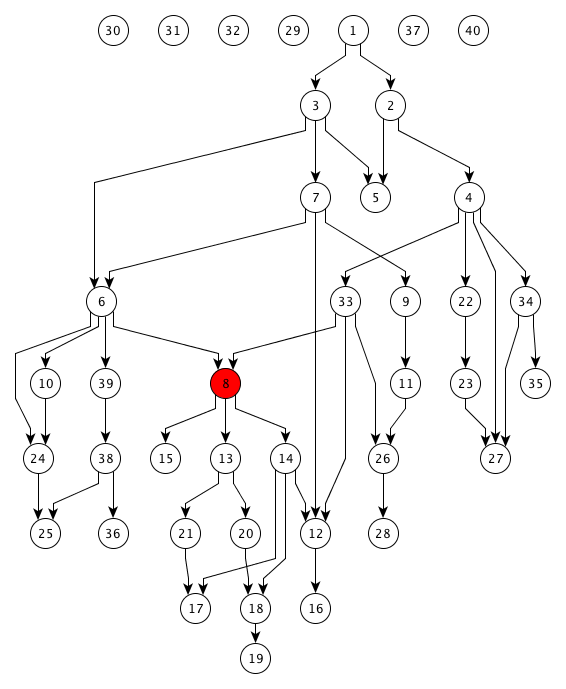
\includegraphics[scale=0.3]{pictures/subgraph_extraction_algorithm_step_1.png}
}
\subfloat[Extract sub-graph for selected node]{
    \label{fig:step_2}
    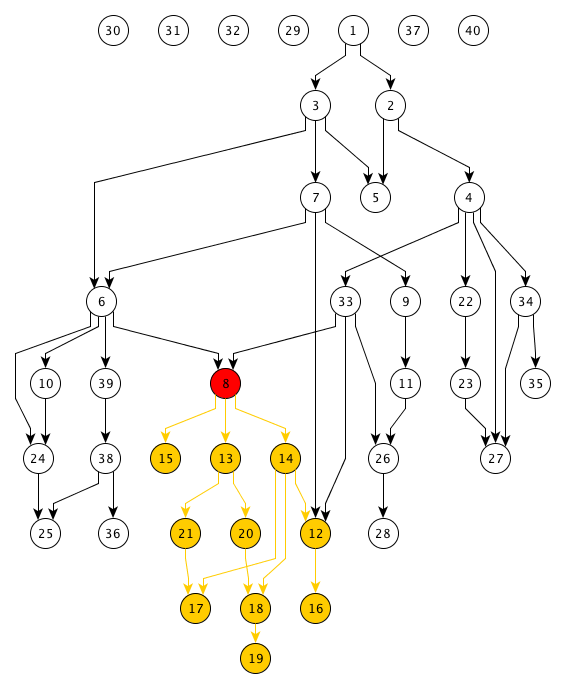
\includegraphics[scale=0.3]{pictures/subgraph_extraction_algorithm_step_2.png}
}
\caption{Sub-graph extraction from the Gene Ontology}
\end{figure}

\item Interactively select node in the Gene Ontology graph (Figure~\ref{fig:step_1}).

\item When node is selected in the Gene Ontology program computes all successors (Figure~\ref{fig:step_2}).

\item Extract leafs from successors (Figure~\ref{fig:step_3}).

\begin{figure}[h!]
\centering
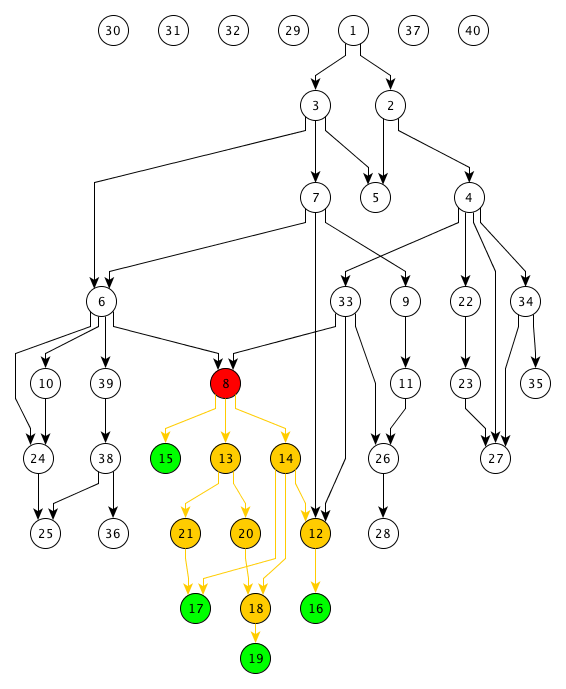
\includegraphics[scale=0.5]{pictures/subgraph_extraction_algorithm_step_3.png}
\caption{Extract leafs from the Gene Ontology sub-graph}
\label{fig:step_3}
\end{figure}

\item Founded sub tree cached. This sub tree is highlighted in cluster analysis tree.

\item Then the program searches corresponded leaves in cluster analysis result tree by label as seen in Figure~\ref{fig:step_4}.

\item For this leaves the program founds root connected to all leaves and extract corresponding sub trees (Figure~\ref{fig:step_5}).
\end{enumerate}

\begin{figure}[h!]
\centering
\subfloat[Find corresponded leafs]{
    \label{fig:step_4}
    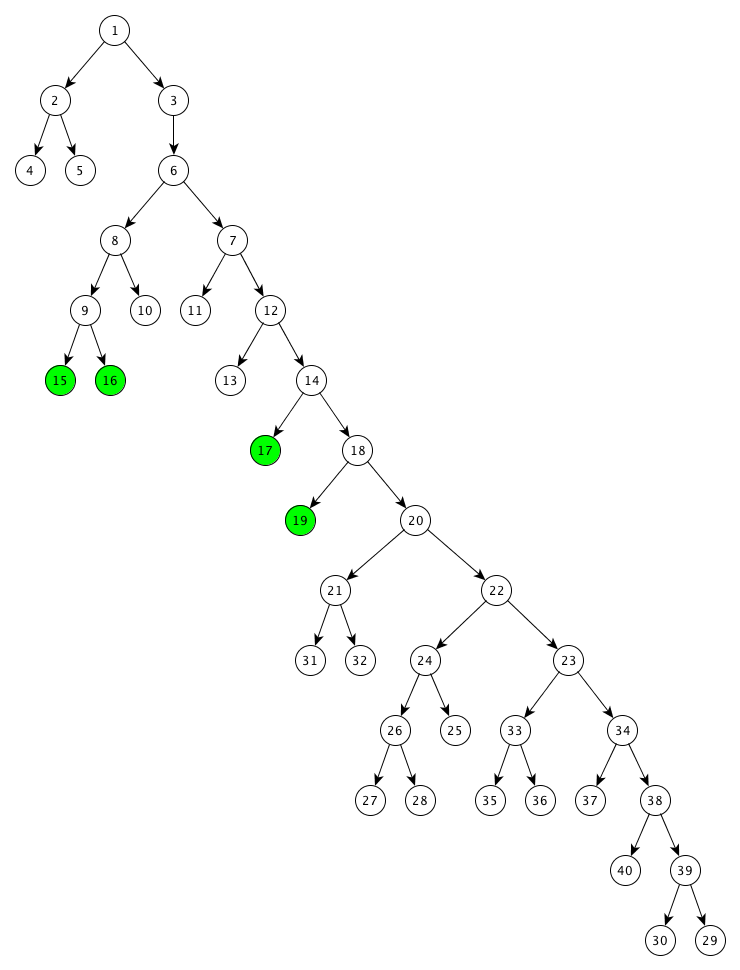
\includegraphics[scale=0.23]{pictures/subgraph_extraction_algorithm_step_4.png}
}
\subfloat[Build sub-graph]{
    \label{fig:step_5}
    
    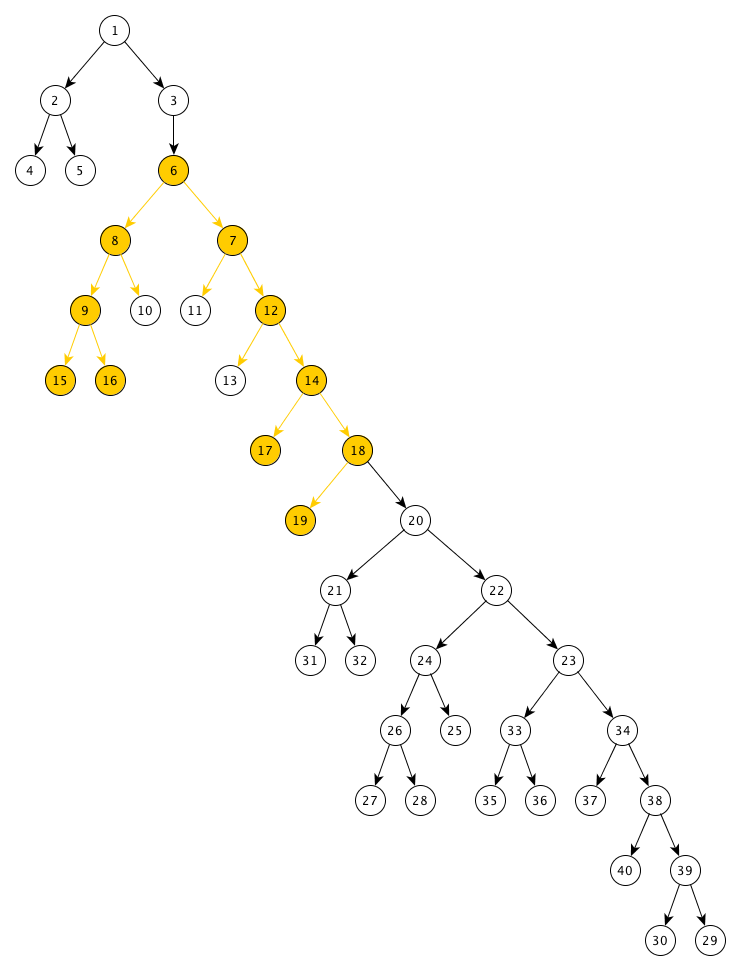
\includegraphics[scale=0.23]{pictures/subgraph_extraction_algorithm_step_5.png}
}
\caption{Analise Cluster graph}
\end{figure}


The aim of the work is to provide flexible tool specially made for biology scientists to deal with huge data sets. Trace relations, as was discussed earlier, in the two separated datasets (Gene Ontology graph and cluster analysis result tree): both graphs are stored separately in the different files. Also during program design we should consider that cluster analysis results graph was produced from Gene Ontology graph using separate tool and clustering algorithm specific to the purpose, that means there are various cluster graphs for the same Gene Ontology.

Provide effective space filling visualization method and allow interactive relations highlighting. The tool also provides ability to track throw graphs discovering: focused or selected vertices labels for both graphs separately, Gene Ontology levels. 

Considering end-user requirements there is use case specific for biology scientist -- interest in the concrete gene in the Gene Ontology; provide search mechanism to find specific gene by name and view it.


\subsection{Dataset Description}
\label{sec:dataset_description}
Gene Ontology data and cluster analysis results presented as directed graphs. They are stored in separate files in special format -- GML files. GML file format covered in the next section.


GO graph is directed acyclic graph has 10,042 vertices and  24,155 edges. It has 1 root, 2,729 nodes and 7,312 leafs (terminal nodes). Figure~\ref{fig:yed_GO_vis} shows visualization of the Gene Ontology graph using Hierarchical layout by yEd~\cite{yed} graph editing tool. It obviously shows imperfectness of classic visualization of the graphs.


\begin{figure}[h!]
\centering
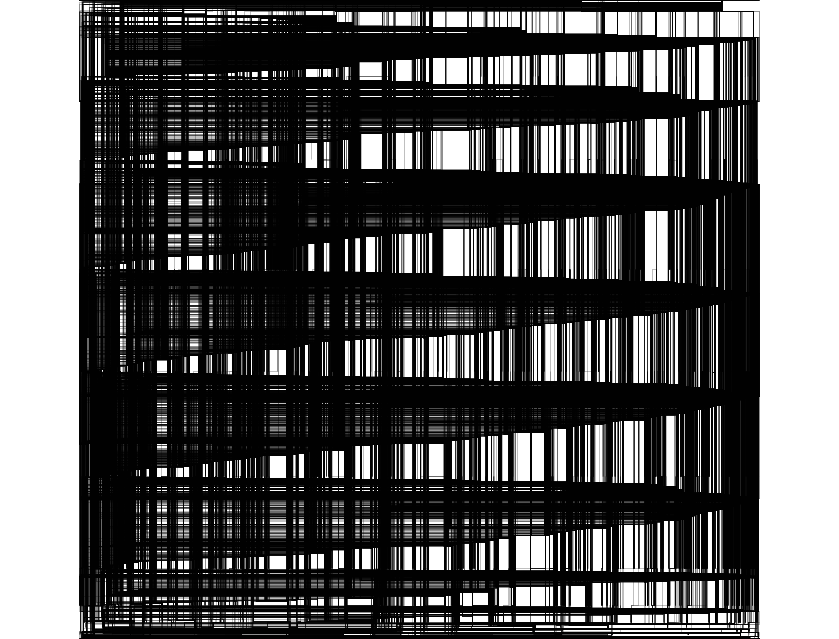
\includegraphics[scale=0.3]{pictures/yEd_GO.png}
\caption{Gene Ontology yEd visualization}
\label{fig:yed_GO_vis}
\end{figure}


Cluster graph is directed binary  tree has 14,623 nodes and 14,622 edges. Cluster graph as a tree has single root, 7,310 nodes and 7,312 leafs. To get an impression of the graph Figure~\ref{fig:Cytoscape_Cluster_1} shows a cluster tree using Cytoscape~\cite{Cytoscape} visualization tool.

\begin{figure}[h!]
\centering
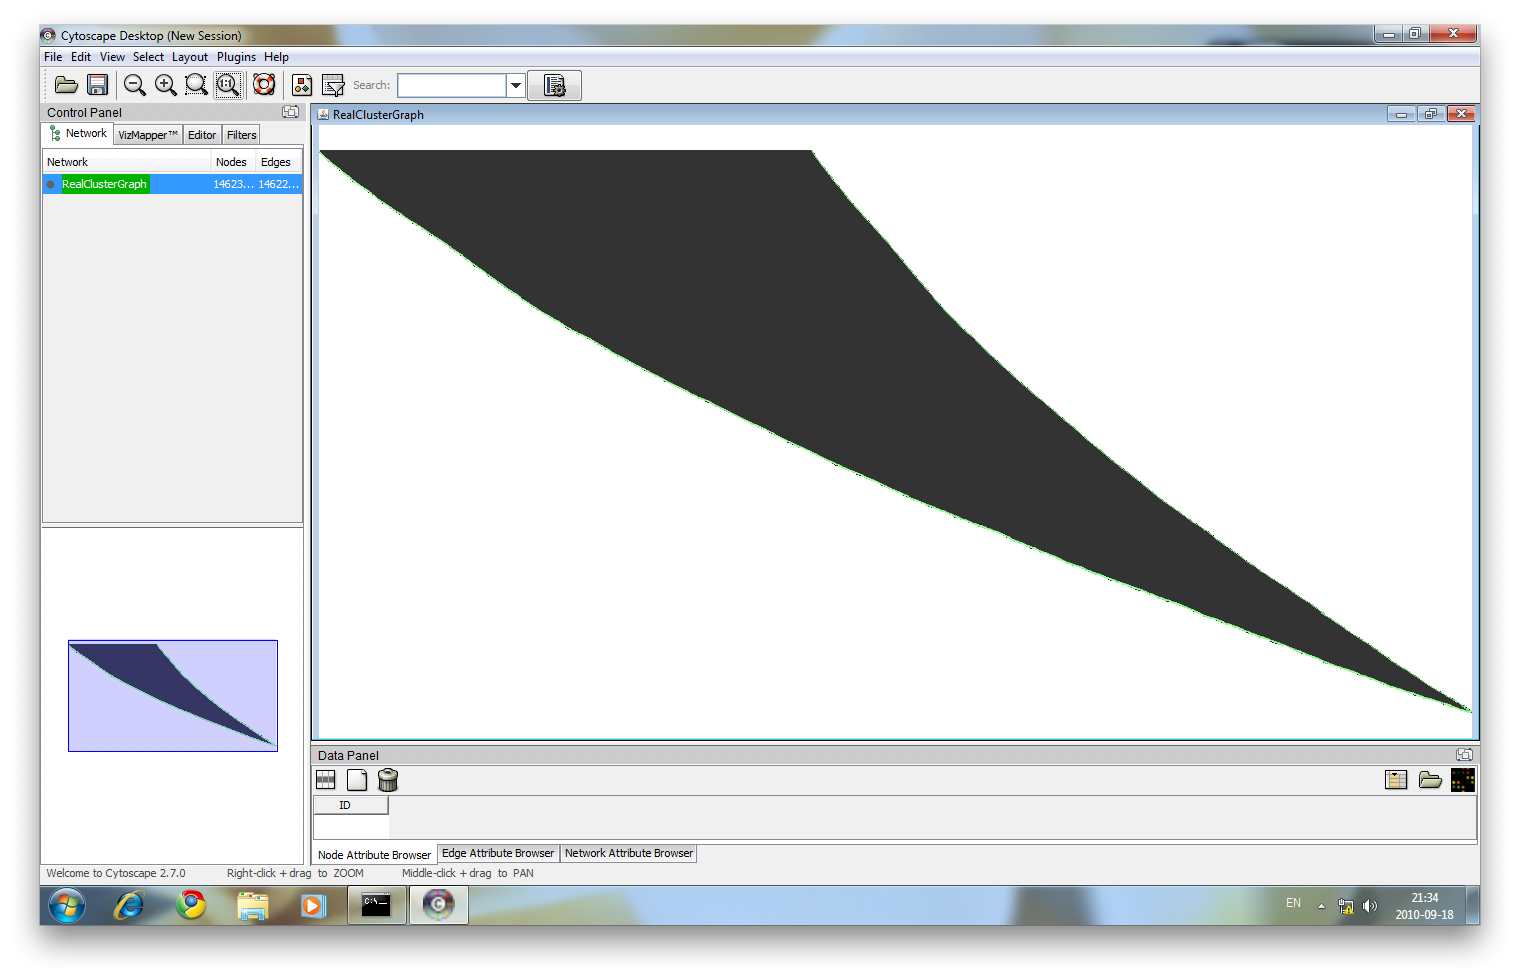
\includegraphics[scale=0.25]{pictures/Cytoscape_cluster_graph_1.png}
\caption{Cluster analysis result tree Cytoscape visualization tool}
\label{fig:Cytoscape_Cluster_1}
\end{figure}

\begin{figure}[h!]
\centering
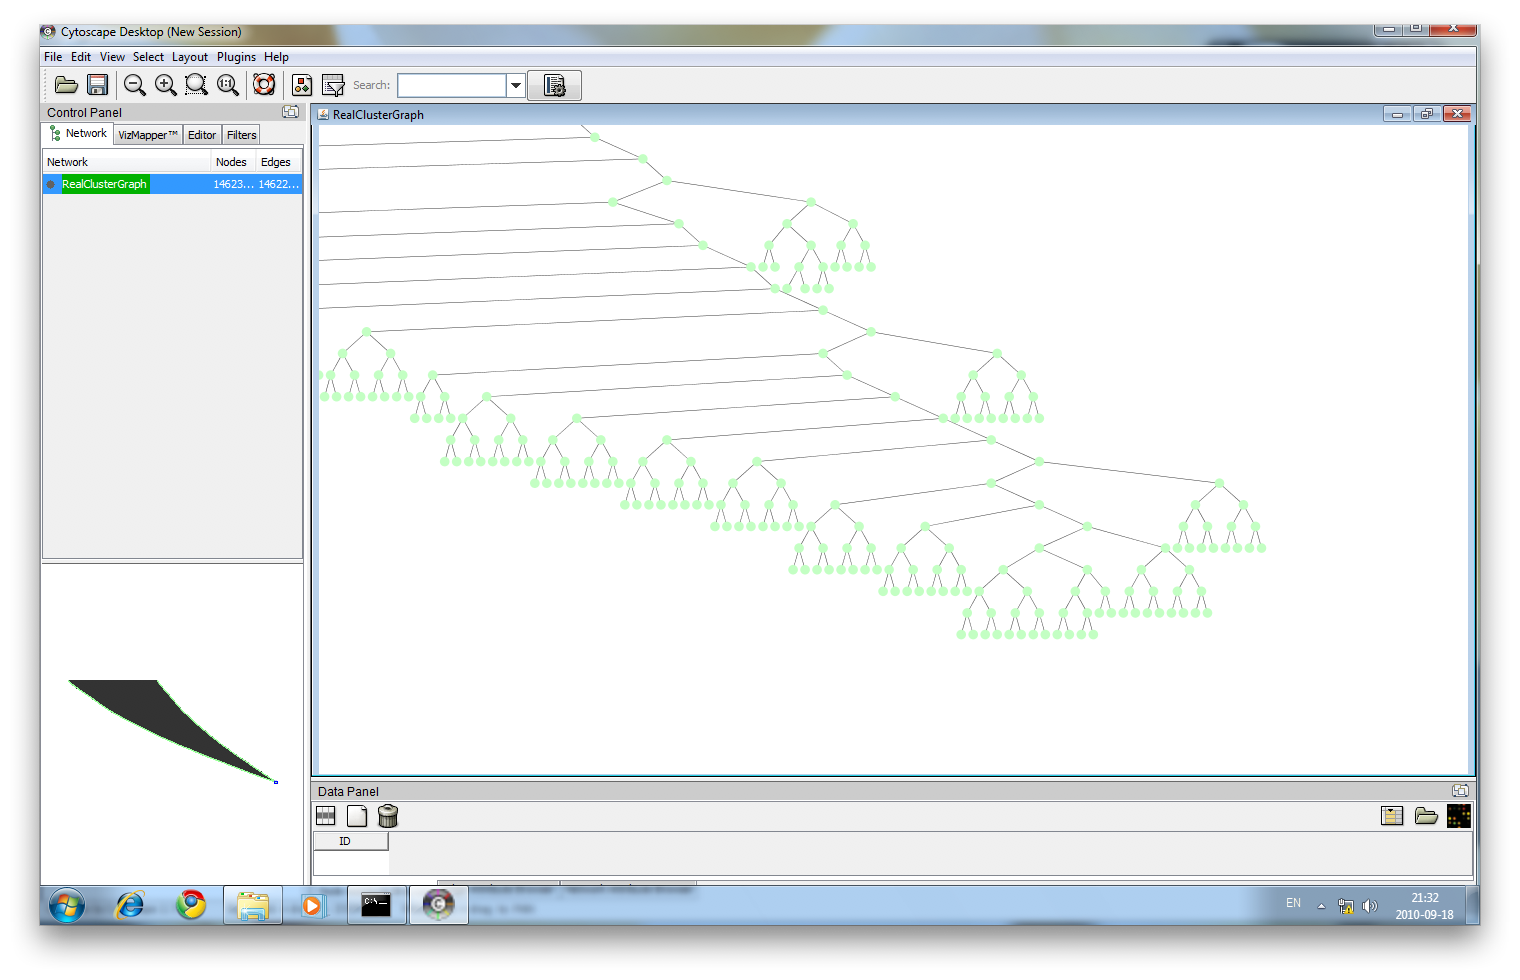
\includegraphics[scale=0.25]{pictures/Cytoscape_cluster_graph_2.png}
\caption{Zoomed cluster analysis result tree}
\label{fig:Cytoscape_Cluster_2}
\end{figure}

Both graphs are independent from each other from developer point of view: they have different node ids and edge ids. But they are corresponded by graph node labels -- both of this graphs have same label for terminal (leaf) graph nodes. This property is used in the sub graph extracting algorithm.


The application should work with large quantity of data over tens of thousands that is why performance is one of the main requirements. It is important to give a consideration on optimization.

\subsection{GML Graph File Format}
 ,,GML, the Graph Modeling Language, is our proposal for a portable file format for graphs. GML's key features are portability, simple syntax, extensibility and flexibility. A GML file consists of a hierarchical key-value lists. Graphs can be annotated with arbitrary data structures. The idea for a common file format was born at the GD'95; this proposal is the outcome of many discussions. GML is the standard file format in the Graphlet~cite{Graphlet} graph editor system. It has been overtaken and adapted by several other systems for drawing graphs."~\cite{GML}


GML format is platform independent, and easy to implement. Furthermore, it has the capability to represent arbitrary data structures, since advanced programs have the need to attach their specific data to nodes and edges. GML is flexible enough that a specific order of declarations is not needed, and that any non-essential data may be omitted. Simple graph is showed in the Listing~\ref{sample_graph_gml}

\begin{center}
	\lstinputlisting[language=xml, tabsize=2, caption={GML description of sample graph}, label={sample_graph_gml}]{graphs/SampleGraph.gml}
\end{center}

Figure~\ref{fig:sample_graph_yed_vis} shows manual visualization of the sample graph using yEd~\cite{yed} graph visualization tool.

\begin{figure}[h!]
\centering
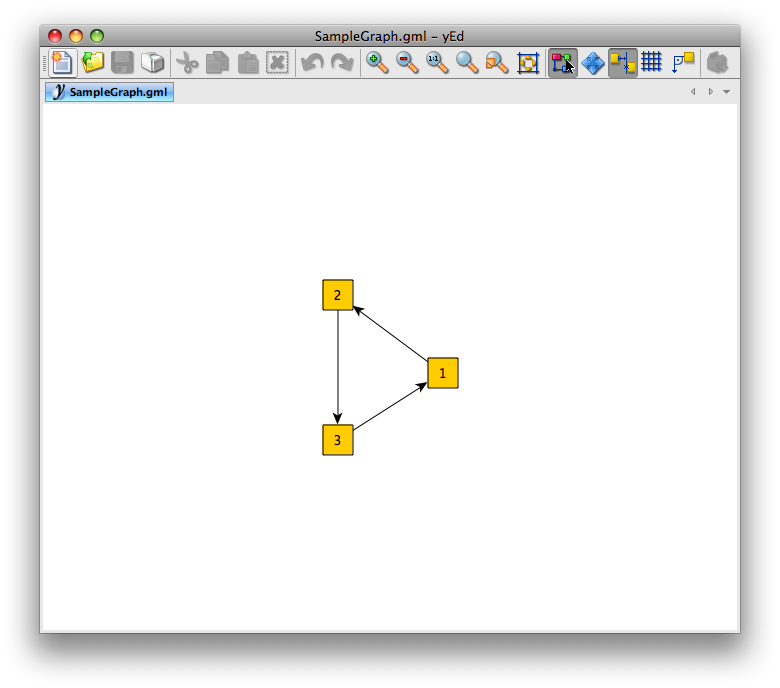
\includegraphics[scale=0.5]{pictures/SampleGraph.png}
\caption{Manual visualization of the sample graph}
\label{fig:sample_graph_yed_vis}
\end{figure}

Listing of the more complex graph with additional properties and is in the Appendix~A and the visualization of this graph showed in Figure~\ref{fig:yed_graph_vis}

\begin{figure}[h!]
\centering
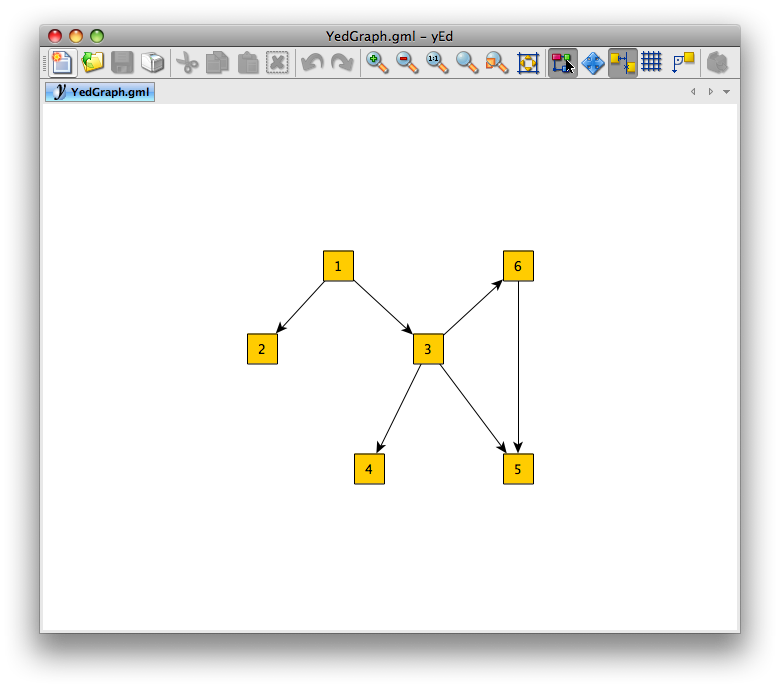
\includegraphics[scale=0.5]{pictures/YedGraph.png}
\caption{Manual visualization of the sample graph}
\label{fig:yed_graph_vis}
\end{figure}

Applications supporting GML~\cite{GML_wiki}

\begin{itemize}
\item Clairlib~\cite{clairlib}, a suite of open-source Perl modules intended to simplify a number of generic tasks in natural language processing (NLP), information retrieval (IR), and network analysis (NA).
\item Cytoscape~\cite{Cytoscape}, an open source bioinformatics software platform for visualizing molecular interaction networks, loads and save previously-constructed interaction networks in GML.
\item NetworkX~\cite{NetworkX}, an open source Python library for studying complex graphs.
\item ocamlgraph\cite{ocamlgraph}, a graph library for OCaml.
\item OGDF\cite{OGDF}, the Open Graph Drawing Framework, an open source C++ library containing implementations of various graph drawing algorithms. The library is self contained; optionally, additional packages like LP-solvers are required for some implementations.
\item Tulip~\cite{Tulip} (software) is a free software in the domain of information visualization capable of manipulating huge graphs (with more than 1.000.000 elements).
\item yEd~\cite{yed}, a free Java-based graph editor, supports import from and export to GML.
\end{itemize}

\subsection{Other Graph File Formats}

\subsubsection{GraphML}
GraphML is a comprehensive and easy-to-use file format for graphs. It consists of a language core to describe the structural properties of a graph and a flexible extension mechanism to add application-specific data.~\cite{GraphML} Its main features include support of:
\begin{itemize}
\item directed, undirected, and mixed graphs;
\item hyper graphs;
\item hierarchical graphs;
\item graphical representations;
\item references to external data;
\item application-specific attribute data;
\item light-weight parsers;
\end{itemize}

The GraphML document consists of a graphml element and a variety of sub elements: graph, node, edge. Figure~\ref{fig:simple_graphml} below is a simple graph. It contains 11 nodes and 12 undirected edges.

\begin{figure}[h!]
\centering
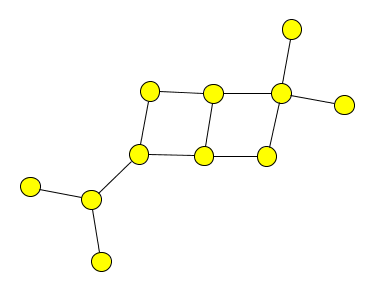
\includegraphics[scale=1.0]{pictures/simple.png}
\caption{A simple graph}
\label{fig:simple_graphml}
\end{figure}


And a corresponded graphml file is showed in Listing~\ref{simple_graphml_file}

\begin{center}
\begin{lstlisting} [language=xml, tabsize=2, caption={Simple graphml file},label=simple_graphml_file]
<graphml>
  <graph id="G" edgedefault="undirected">
    <node id="n0"/>
    <node id="n1"/>
    <node id="n2"/>
    <node id="n3"/>
    <node id="n4"/>
    <node id="n5"/>
    <node id="n6"/>
    <node id="n7"/>
    <node id="n8"/>
    <node id="n9"/>
    <node id="n10"/>
    <edge source="n0" target="n2"/>
    <edge source="n1" target="n2"/>
    <edge source="n2" target="n3"/>
    <edge source="n3" target="n5"/>
    <edge source="n3" target="n4"/>
    <edge source="n4" target="n6"/>
    <edge source="n6" target="n5"/>
    <edge source="n5" target="n7"/>
    <edge source="n6" target="n8"/>
    <edge source="n8" target="n7"/>
    <edge source="n8" target="n9"/>
    <edge source="n8" target="n10"/>
  </graph>
</graphml>
\end{lstlisting}
\end{center}

\subsubsection{DOT Graph File Format}
DOT is a plain text graph description language. It is a simple way of describing graphs in human readable form.

,,DOT graphs are typically files that end with the .gv (or .dot) extension. At its simplest, DOT can be used to describe an undirected graph. An undirected graph shows simple relations between objects, such as friendship between people. The graph keyword is used to begin a new graph, and nodes are described within curly braces. A double-hyphen (-\ -) is used to show relations between the nodes."~\cite{DOT}

\begin{center}
\begin{lstlisting} [language=C, tabsize=2, caption={DOT file format: undirected graph}]
graph graphname {
     a - - b - - c;
     b - - d;
}
\end{lstlisting}
\end{center}

,,Similar to undirected graphs, DOT can describe directed graphs, such as flowcharts and dependency trees. The syntax is the same as for undirected graphs, except the digraph keyword is used to begin the graph, and an arrow ($->$) is used to show relationships between nodes."~\cite{DOT}

\begin{center}
\begin{lstlisting} [language=C, tabsize=2, caption={DOT file format: directed graph}]
graph graphname {
     a -> b -> c;
     b -> d;
}
\end{lstlisting}
\end{center}

Visual representation of both graphs showed Figure~\ref{fig:dot_graphs} below.

\begin{figure}[h!]
\centering
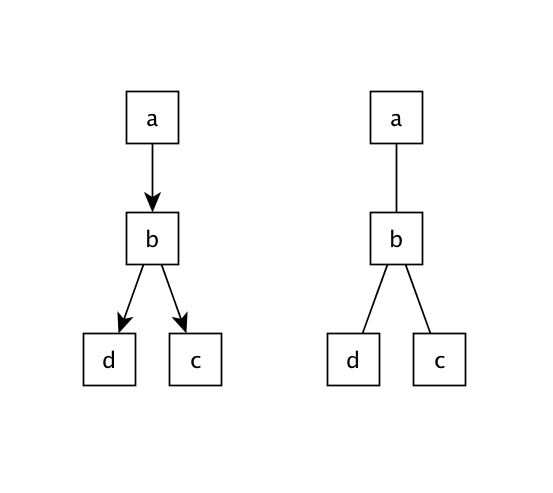
\includegraphics[scale=0.3]{pictures/dot_graph.png}
\caption{Directed and undirected graphs}
\label{fig:dot_graphs}
\end{figure}

\subsubsection{DGML}
DGML is an XML-based file format for directed graphs. Here is what a simple directed graph with three nodes and two links between them looks like

\begin{center}
\begin{lstlisting} [language=XML, tabsize=2, caption={DGML file format}]
<?xml version='1.0' encoding='utf-8'?>
<DirectedGraph xmlns="http://schemas.microsoft.com/vs/2009/dgml">
  <Nodes>
    <Node Id="a" Label="a" Size="10" />
    <Node Id="b" Background="#FF008080" Label="b" />
    <Node Id="c" Label="c" Start="2010-06-10" />
  </Nodes>
  <Links>
    <Link Source="a" Target="b" />
    <Link Source="a" Target="c" />
  </Links>
  <Properties>
    <Property Id="Background" Label="Background" DataType="Brush" />
    <Property Id="Label" Label="Label" DataType="String" />
    <Property Id="Size" DataType="String" />
    <Property Id="Start" DataType="DateTime" />
  </Properties>
</DirectedGraph>
\end{lstlisting}
\end{center}

The complete XSD schema for DGML is available at~\url{http://schemas.microsoft.com/vs/2009/dgml/}. DGML not only allows describing nodes and links in a graph, but also annotating those nodes and links with any user defined property and/or category.

\subsubsection{GXL}
GXL (Graph eXchange Language) is an XML based exchange format for several kinds of graph information. GXL provides a standardized notation for exchanging instance data (graph) including their structure (graph schema).

,,GXL was created to fulfill the need to exchange data between re-engineering tools. Previously, interoperability between tools relied on converters between local formats. This approach requires case-by-case negotiation of exchange semantics. As the research area matured, it became apparent that a standard exchange format was needed and that this format should provide a mechanism to help articulate semantics.''~\cite{GXL}.

\subsubsection{SVG}
SVG is open graphical data storage format. Has been in development since 1999 by a group of companies within the W3C. SVG drew on experience from the designs of two older formats: Precision Graphics Markup Language (PGML) developed from Adobe's PostScript and Vector Markup Language (VML) developed from Microsoft's RTF. Which were submitted to W3C in 1998.


SVG allows three types of graphic objects:
\begin{itemize}
\item Vector graphics
\item Raster graphics
\item Text
\end{itemize}

,,Graphical objects, including PNG and JPEG raster images, can be grouped, styled, transformed, and composited into previously rendered objects. SVG does not directly support z-indices that separate drawing order from document order for overlapping objects, unlike some other vector mark up languages like VML. Text can be in any XML name space suitable to the application, which enhances search ability and accessibility of the SVG graphics. The feature set includes nested transformations, clipping paths, alpha masks, filter effects, template objects and extensibility..''~\cite{SVG}
